%\setbeamertemplate{footline}[frame number]
\begin{frame}
\frametitle{Motivation}
$\Omega \subset \mathbb{R}^2$: smooth connected domain,
$\mathcal{H}$ : Hilbert space, $\mathcal{K}_g$ : convex set.
\\
\vspace*{0.1 cm}
$a: \mathcal{H} \times \mathcal{H} \rightarrow \mathbb{R}$: bilinear continuous  coercive form, $\ell : \mathcal{H} \rightarrow \mathbb{R}$ : linear continuous form
\begin{equation*}
\text{Find} \quad \textcolor{red}{u} \in \mathcal{K}_g \quad a(\textcolor{red}{u},v-\textcolor{red}{u}) \geq \ell(v-\textcolor{red}{u}) \quad \forall v \in \mathcal{K}_g
\end{equation*}
\invisible<1>{
\textcolor{cadmiumgreen}{\textbf{Application to several problems in contact mechanics}}
\\
\vspace*{0.2 cm}
\invisible<2>{
\textcolor{midnightblue}{\textbf{Obstacle problem:}}
Find $\textcolor{red}{u} \in \Kg := \left\{ v \in H^1(\Omega) \ \text{s.t.} \ v=g \ \text{on} \ \partial \Omega , \ \text{and} \ v \geq \Psi \ \text{in} \ \Omega \right\}$ such that
\begin{equation*}
\left( \nab \textcolor{red}{u}, \nab (v-\textcolor{red}{u}) \right)_{\Omega} \geq \left(f,v-\textcolor{red}{u}\right)_{\Omega} \quad \forall v \in \Kg
\end{equation*}
\vspace*{-0.2 cm}
\begin{minipage}{0.55\linewidth}
\begin{itemize}
\item $\textcolor{red}{u}$: displacement of an elastic membrane
  \item $\Psi \in H^1(\Omega)$: position of the lower obstacle 
  \item $g \in H^{\frac{1}{2}}(\partial \Omega)$: Dirichlet boundary datum for $\textcolor{red}{u}$
    \item $f \in L^2(\Omega)$: force acting on the membrane
\end{itemize}
\end{minipage}
\hfill
\begin{minipage}{0.4\linewidth}
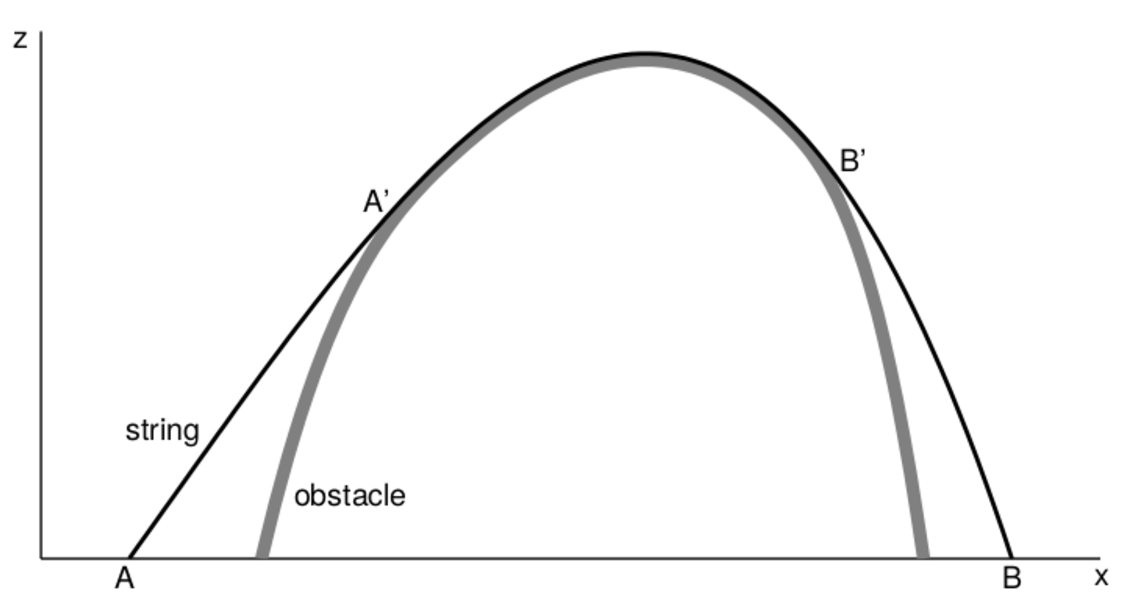
\includegraphics[scale=0.3]{image_obstacle}
\end{minipage}

\invisible<3>{
}}}
\end{frame}
%%%%%%%%%%%%
\begin{frame}
  \textcolor{midnightblue}{\textbf{Signorini problem:}}
  $\partial \Omega = \Gamma_{\mathrm{D}} \cup \Gamma_{\mathrm{N}} \cup \Gamma_{\mathrm{C}}$. \\
  $\Gamma_{\mathrm{D}}$: Dirichlet boundary conditions, $\Gamma_{\mathrm{N}}$: Neumann boundary conditions \\
  $\Gamma_{\mathrm{C}}$: Unilateral contact boundary conditions
  \\
  \vspace*{0.1 cm}
  Find $\textcolor{red}{\bu} \in \Kg := \left\{ \bv \in [H^1(\Omega)]^2 \ \text{s.t.} \ \bv=g \ \text{on} \ \Gamma_{\mathrm{D}}, \ \text{and} \ \bv\cdot \bn \leq 0 \ \text{on} \ \Gamma_{\mathrm{C}} \right\}$ such that
\begin{equation*}
\left( \sigma (\textcolor{red}{\bu}), \epsilon (\bv-\textcolor{red}{\bu}) \right)_{\Omega} \geq \left(\bbf,\bv-\textcolor{red}{\bu}\right)_{\Omega} + \left({\bm g}_{N}, \bv-\textcolor{red}{\bu} \right)_{\Gamma_{\mathrm{N}}}\quad \forall \bv \in \Kg
\end{equation*}

\begin{minipage}{0.55 \linewidth}
\begin{itemize}
\item $g \in H^{\frac{1}{2}}(\Gamma_{\mathrm{D}})$ : Dirichlet boudary datum for $\textcolor{red}{u}$
  \item  ${\bm g}_{\mathrm{N}} \in [L^2(\Gamma_{\mathrm{N}})]^2$ :  Neumann boundary data
  \item  $f \in [L^2(\Omega)]^2$: force acting on the solid elastic.
\end{itemize}
\end{minipage}
\hfill
\begin{minipage}{0.42 \linewidth}
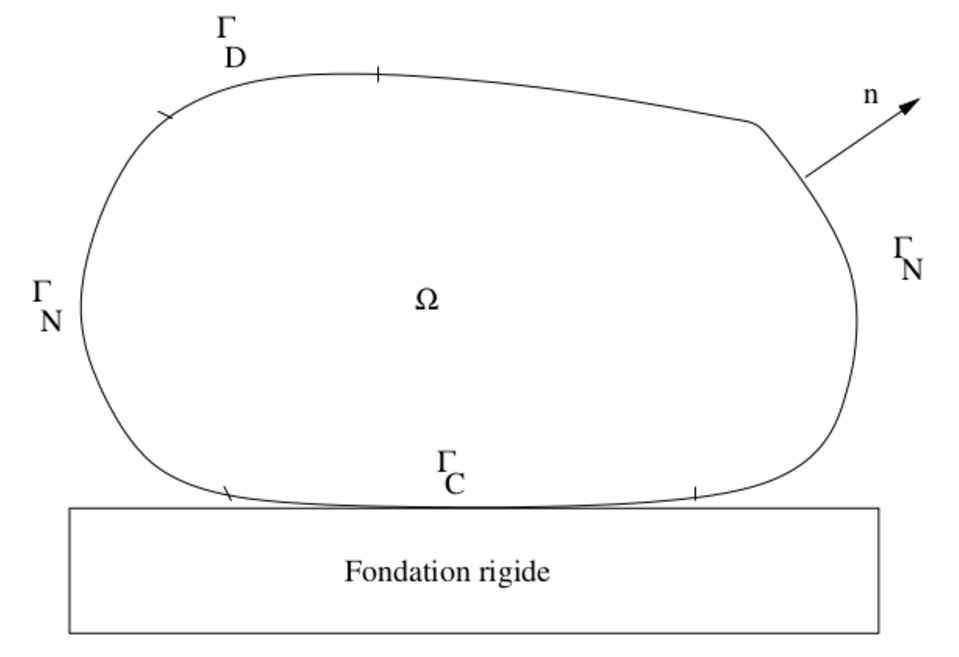
\includegraphics[scale=0.4]{image_signorini}
\end{minipage}
\end{frame}
\begin{frame}
\textcolor{midnightblue}{\textbf{Contact between two membranes:}}
\\
\vspace*{0.1 cm}
Find $\textcolor{red}{\bu}:=(\textcolor{red}{u_1},\textcolor{red}{u_2}) \in \Kg := \left\{ \bv = \left(v_1,v_2\right) \in H_{g_1}^1(\Omega) \times H_{g_2}^1(\Omega) \ \text{s.t.} \ v_1 - v_2 \geq 0  \ \text{a.e.} \ \text{in} \ \Omega \right\}$ such that
 \begin{equation*}
  \fbox{$ \sum_{\alpha=1}^2 \mu_{\alpha}
   \left( \nab \textcolor{red}{u_{\alpha}}, \nab \left(v_{\alpha} - \textcolor{red}{u_{\alpha}} \right) \right)_{\Omega} \geq
   \sum_{\alpha=1}^2 \left(f_{\alpha}, v_{\alpha} - \textcolor{red}{u_{\alpha}} \right)_{\Omega} \quad \forall \bv \in \Kg$ }
 \end{equation*}
 \begin{minipage}{0.37 \linewidth}
 \begin{itemize}
 \item $\mu_1, \mu_2$: tensions of the membranes
   \item $g_1 \geq g_2$ : boundary data
\end{itemize} 
 \end{minipage}
 \hfill
 \begin{minipage}{0.55 \linewidth}
\begin{figure}
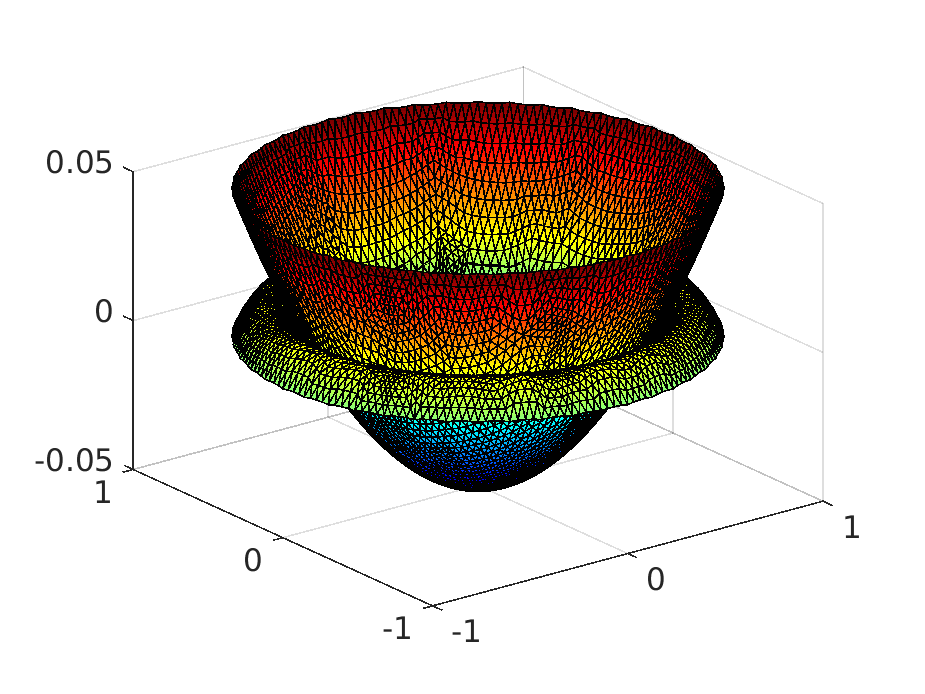
\includegraphics[scale = 0.5]{fig_article_chap_1/fig_membrane_cv.eps}    
\end{figure}
\end{minipage}

 \end{frame}
%%%%

%%%%%%%%%%%%%%%%%
\begin{frame}
\vspace*{0.1 cm}
\textcolor{red}{\textbf{Study the contact problem between two membranes}}
\\
\vspace{0.3 cm}
\textcolor{cadmiumgreen}{\textbf{Propose robust algorithms}}
\begin{itemize}
\item Discretization by the finite element method, the discontinuous Galerkin method, the hybrid high-order method
\end{itemize}
\textcolor{cadmiumgreen}{\textbf{Nonlinear resolution}}
\begin{itemize}
\item Semismooth Newton methods
  \end{itemize}
\textcolor{cadmiumgreen}{\textbf{Quantify the error}}
\begin{itemize}
  \item A posteriori error estimates
  \item Distinction of each error components
\end{itemize}

\textcolor{cadmiumgreen}{\textbf{Save computational time}}
\begin{itemize}
\item Adaptivity
  \end{itemize}
  \invisible<1>{
  \textcolor{red}{\textbf{Extension to unsteady problems?}}
  \invisible<2>{
  }}
\end{frame}
